\documentclass{beamer}

\usetheme{Madrid}

\usepackage{amsmath, amssymb}
\usepackage{tikz}
\usetikzlibrary{arrows.meta, positioning, matrix}

\title{Semirings for database provenance}
\author{Yiannis Hadjicharalambous}
\date{4 June 2026}

\begin{document}


\begin{frame}
  \titlepage
\end{frame}

\begin{frame}{What is a database?}
  \centering
  % Resizebox ensures the entire diagram fits perfectly within the slide margins
  \resizebox{0.95\textwidth}{!}{%
    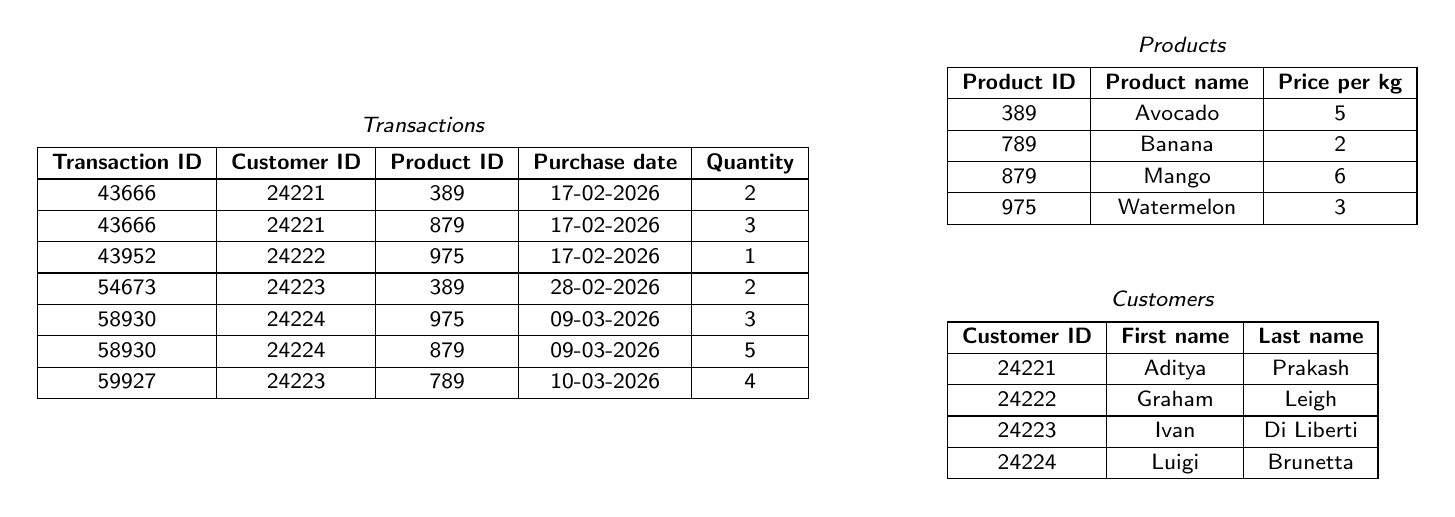
\begin{tikzpicture}[
        node distance=0.6cm and 1.5cm,
        font=\footnotesize\sffamily
      ]

      % Compact table row height and column padding for slide layout
      \renewcommand{\arraystretch}{1.15}
      \setlength{\tabcolsep}{5pt}

      % ==================== TABLES ====================

      \node (Transaction) [align=center] {
        \textit{Transactions} \\[0.15cm]
        \begin{tabular}{|c|c|c|c|c|}
          \hline
          \textbf{Transaction ID} & \textbf{Customer ID} & \textbf{Product ID} & \textbf{Purchase date} & \textbf{Quantity} \\ \hline
          43666                   & 24221                & 389                 & 17-02-2026             & 2                 \\ \hline
          43666                   & 24221                & 879                 & 17-02-2026             & 3                 \\ \hline
          43952                   & 24222                & 975                 & 17-02-2026             & 1                 \\ \hline
          54673                   & 24223                & 389                 & 28-02-2026             & 2                 \\ \hline
          58930                   & 24224                & 975                 & 09-03-2026             & 3                 \\ \hline
          58930                   & 24224                & 879                 & 09-03-2026             & 5                 \\ \hline
          59927                   & 24223                & 789                 & 10-03-2026             & 4                 \\ \hline
        \end{tabular}
      };

      \node (Product) [align=center, right=1.5cm of Transaction.east, anchor=south west, yshift=0.3cm] {
        \textit{Products} \\[0.15cm]
        \begin{tabular}{|c|c|c|}
          \hline
          \textbf{Product ID} & \textbf{Product name} & \textbf{Price per kg} \\ \hline
          389                 & Avocado               & 5                     \\ \hline
          789                 & Banana                & 2                     \\ \hline
          879                 & Mango                 & 6                     \\ \hline
          975                 & Watermelon            & 3                     \\ \hline
        \end{tabular}
      };

      \node (Customer) [align=center, right=1.5cm of Transaction.east, anchor=north west, yshift=-0.3cm] {
        \textit{Customers} \\[0.15cm]
        \begin{tabular}{|c|c|c|}
          \hline
          \textbf{Customer ID} & \textbf{First name} & \textbf{Last name} \\ \hline
          24221                & Aditya              & Prakash            \\ \hline
          24222                & Graham              & Leigh              \\ \hline
          24223                & Ivan                & Di Liberti         \\ \hline
          24224                & Luigi               & Brunetta           \\ \hline
        \end{tabular}
      };

    \end{tikzpicture}%
  }
\end{frame}

\begin{frame}{What is a database?}
  We assume:
  \begin{itemize}
    \item a countably infinite set of constants (values) $\mathbb{D}$, called the \emph{domain}.\pause
    \item a totally ordered countably infinite set $\mathcal{U}$ of \emph{attribute names}. We use the symbols $U,V$ for finite subsets of $\mathcal{U}$.\pause
  \end{itemize}

  We define:

  \begin{itemize}
    \item A \emph{tuple} as a function $t : U \to \mathbb{D}$.\pause
    \item A \emph{relation} $R$ as a finite set of tuples over $U$.\pause
    \item A \emph{database} $D$ as a finite set of relations.
  \end{itemize}
\end{frame}

\begin{frame}{How do we query a database?}
  Relational algebra is an algebraic formalism in which queries are expressed by applying a sequence of operations to relations.\pause

  \bigskip
  
  The \emph{relational algebra} consists of the following operations:
  \begin{itemize}
    \item Selection, $\sigma_\theta(R)$: Keep tuples satisfying condition $\theta$
    \item Projection, $\pi_L(R)$: Keep only attributes $L$
    \item Natural join, $R \bowtie S$: Merge tuples matching on common attributes
    \item Renaming, $\rho_\beta(R)$: Rename attributes according to $\beta$
    \item Union, $R \cup S$: Combine unique tuples
    \item Difference, $R - S$: Keep tuples present in $R$ but not in $S$
  \end{itemize}
\end{frame}

\begin{frame}{Example}
  Find all the times a mango or banana was purchased
\end{frame}

\begin{frame}{What is database provenance?}
  Provenance is a mechanism that relates data in an output to the contributing data in the input. \pause

  \bigskip

  Provenance is typically represented as a form of annotation information, usually by tagging data on the tuple-level of a relation.
\end{frame}


\begin{frame}{What is a semiring?}
\end{frame}

\begin{frame}{Semiring framework}
  Main idea: have the values for the annotations come from a semiring. \pause

  The most general of all being the polynomial semiring $(\mathbb{N}[\mathrm{X}], +, \cdot,0,1)$. \pause

  The provenance for $(a, a)$ from our query from the previous slide would be the polynomial $p^3 + 2pqr$.
\end{frame}

\begin{frame}{Positive relational algebra}
  The original paper translated the following relational algebra operations into the semiring framework with the $+$ and $\cdot$ operations: \pause
  \begin{itemize}
    \item \alt<6->{\textbf{S}}{S}election (filter tuples): $\sigma_\theta(R)$ \pause
    \item \alt<6->{\textbf{P}}{P}rojection (remove/rearrange attributes): $\pi_L(R)$ \pause
    \item \alt<6->{\textbf{C}}{C}artesian product: $R \times S$ \pause
    \item \alt<6->{\textbf{U}}{U}nion (add tuples): $R \cup S$ \pause
  \end{itemize}
\end{frame}

\begin{frame}{Extending the semiring framework}
  Extensive work has been carried out to extend the semiring framework to more expressive query languages with: \pause
  \begin{itemize}
    \item Aggregation \pause
    \item Difference
  \end{itemize}
\end{frame}

\begin{frame}{Aggregate queries}
  \begin{center}
    \resizebox{0.95\textwidth}{!}{
      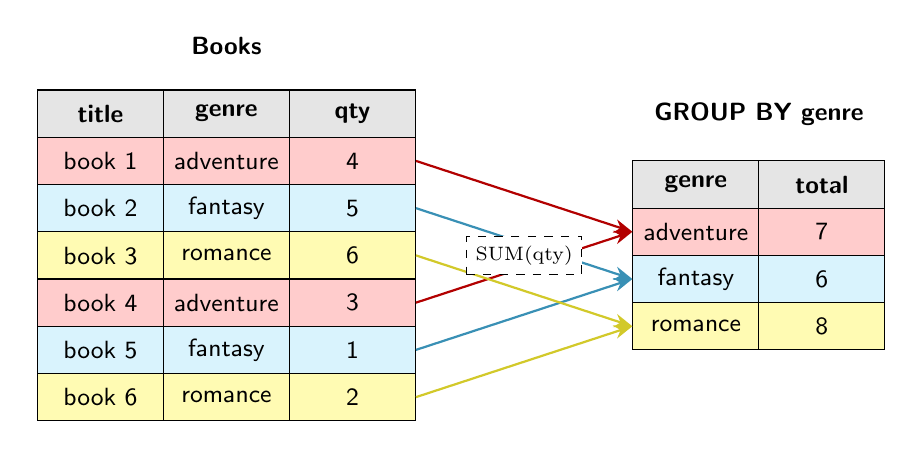
\begin{tikzpicture}[
          font=\sffamily\small,
          cell/.style={draw, minimum height=0.6cm, minimum width=1.6cm, anchor=center, inner sep=2pt},
          header/.style={cell, fill=gray!20, font=\sffamily\bfseries\small},
          % Row colors
          adv/.style={fill=red!20},
          fan/.style={fill=cyan!15},
          rom/.style={fill=yellow!30},
          % Table style
          table/.style={
              matrix of nodes,
              nodes={cell},
              column sep=-\pgflinewidth,
              row sep=-\pgflinewidth,
              nodes in empty cells,
              ampersand replacement=\&
            },
          arrow/.style={-Stealth, thick, rounded corners}
        ]

        % -------- Left Table (Books) --------
        \matrix [table] (L) {
        |[header]| title \& |[header]| genre   \& |[header]| qty \\
        |[adv]| book 1   \& |[adv]| adventure \& |[adv]| 4     \\
        |[fan]| book 2   \& |[fan]| fantasy   \& |[fan]| 5     \\
        |[rom]| book 3   \& |[rom]| romance   \& |[rom]| 6     \\
        |[adv]| book 4   \& |[adv]| adventure \& |[adv]| 3     \\
        |[fan]| book 5   \& |[fan]| fantasy   \& |[fan]| 1     \\
        |[rom]| book 6   \& |[rom]| romance   \& |[rom]| 2     \\
        };

        % -------- Right Table (Aggregation result) --------
        % Reduced horizontal distance from 4cm to 2.5cm to help it fit
        \matrix [table, right=2.5cm of L] (R) {
        |[header]| genre   \& |[header]| total \\
        |[adv]| adventure \& |[adv]| 7     \\
        |[fan]| fantasy   \& |[fan]| 6    \\
        |[rom]| romance   \& |[rom]| 8     \\
        };

        % -------- Labels --------
        \node[above=0.2cm of L] {\textbf{Books}};
        \node[above=0.2cm of R] {\textbf{GROUP BY genre}};

        % -------- Arrows --------
        \begin{scope}
          % Adventure
          \draw[arrow, red!70!black] (L-2-3.east) -- (R-2-1.west);
          \draw[arrow, red!70!black] (L-5-3.east) -- (R-2-1.west);

          % Fantasy
          \draw[arrow, cyan!70!black] (L-3-3.east) -- (R-3-1.west);
          \draw[arrow, cyan!70!black] (L-6-3.east) -- (R-3-1.west);

          % Romance
          \draw[arrow, yellow!80!black] (L-4-3.east) -- (R-4-1.west);
          \draw[arrow, yellow!80!black] (L-7-3.east) -- (R-4-1.west);

          % Logical operator label
          \node[draw, dashed, fill=white, font=\scriptsize] at ([xshift=1.25cm]L.east) {SUM(qty)};
        \end{scope}

      \end{tikzpicture}
    } % End of \resizebox
  \end{center}
\end{frame}

\begin{frame}{Aggregation provenance}

\end{frame}

\begin{frame}{Difference in provenance}

\end{frame}


\begin{frame}{Approaches to difference}
  Several researchers proposed different ways to define difference on semiring-based databases. \pause
  \begin{itemize}
    \item Specifying a set of equations \pause
    \item Monus operation on naturally ordered semirings \pause
    \item Quotient constructions
  \end{itemize}
\end{frame}

\begin{frame}{Open challenges}
  \pause
  \begin{itemize}
    \item Unified framework for recursion, aggregates, and difference \pause
    \item Trade-offs between generality and usability \pause
    \item Limits of semiring-based provenance
  \end{itemize}
\end{frame}

\end{document}